\section{ASSISTANT SE Use Case}

\begin{frame}
\frametitle{An Industrial Example}
\begin{itemize}
\item ASSISTANT project Siemens Energy use case
\item Mid/Long-term scheduling/production planning
\item Realistic/not real data
\item Rather complex constraint model
\begin{itemize}
\item Multi-stage BOM
\item Alternative Process Paths
\item Alternative machines
\item Quality/cost based routing preferences
\item Potential outsourcing of certain steps
\item Machine specific calendars
\item Infeasible release/due date pairs
\item Calendar dependent speed reduction
\item Complex manpower constraints  
\end{itemize}
\end{itemize}
\end{frame}


\begin{frame}
\frametitle{Assistant Siemens Energy Use Case}
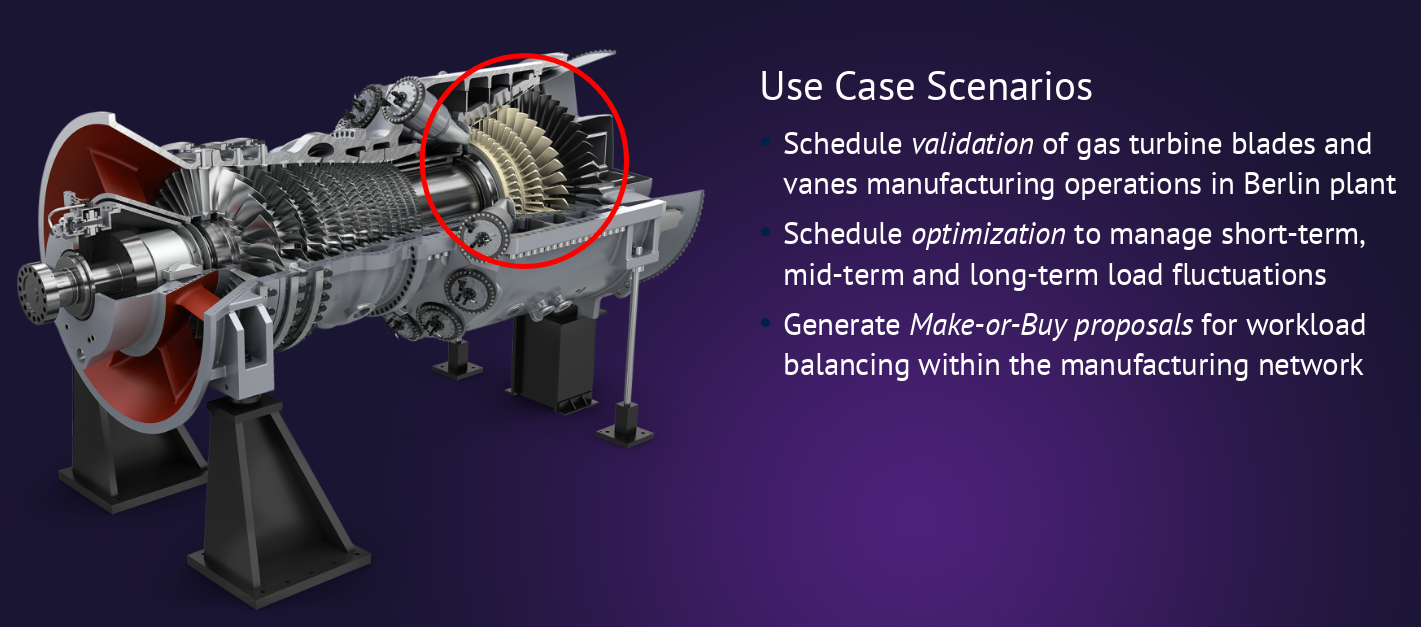
\includegraphics[width=\textwidth]{imagesse/assistantgasturbine}
\end{frame}

\begin{frame}
\frametitle{Digital Twin}
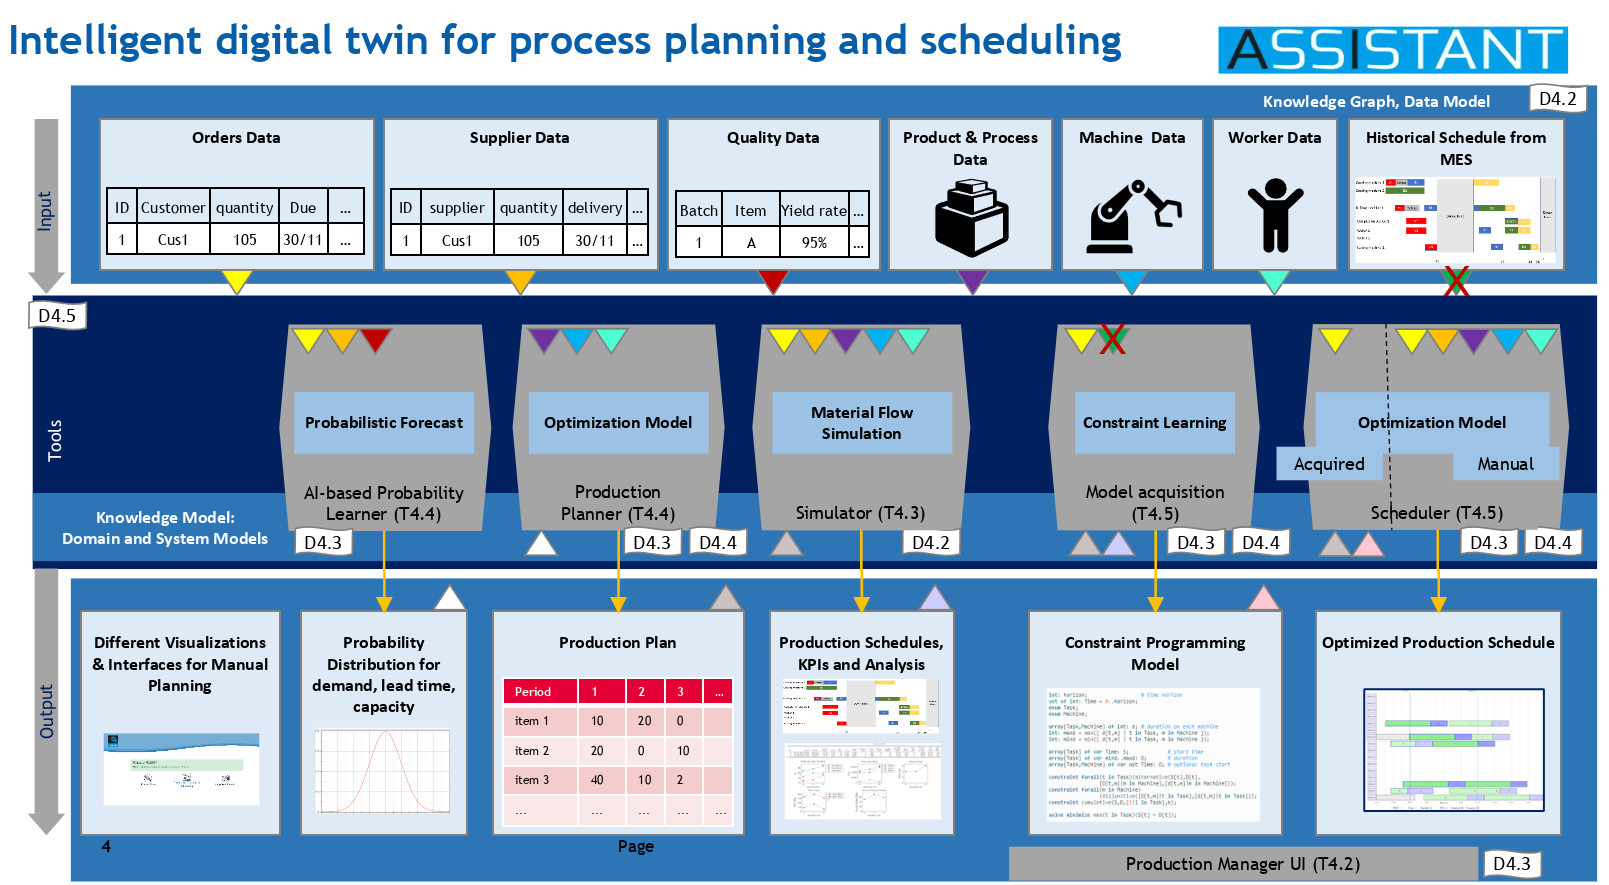
\includegraphics[width=.9\textwidth]{imagesse/assistantdigitaltwin}
\end{frame}

\begin{frame}
\frametitle{SE Product Routing}
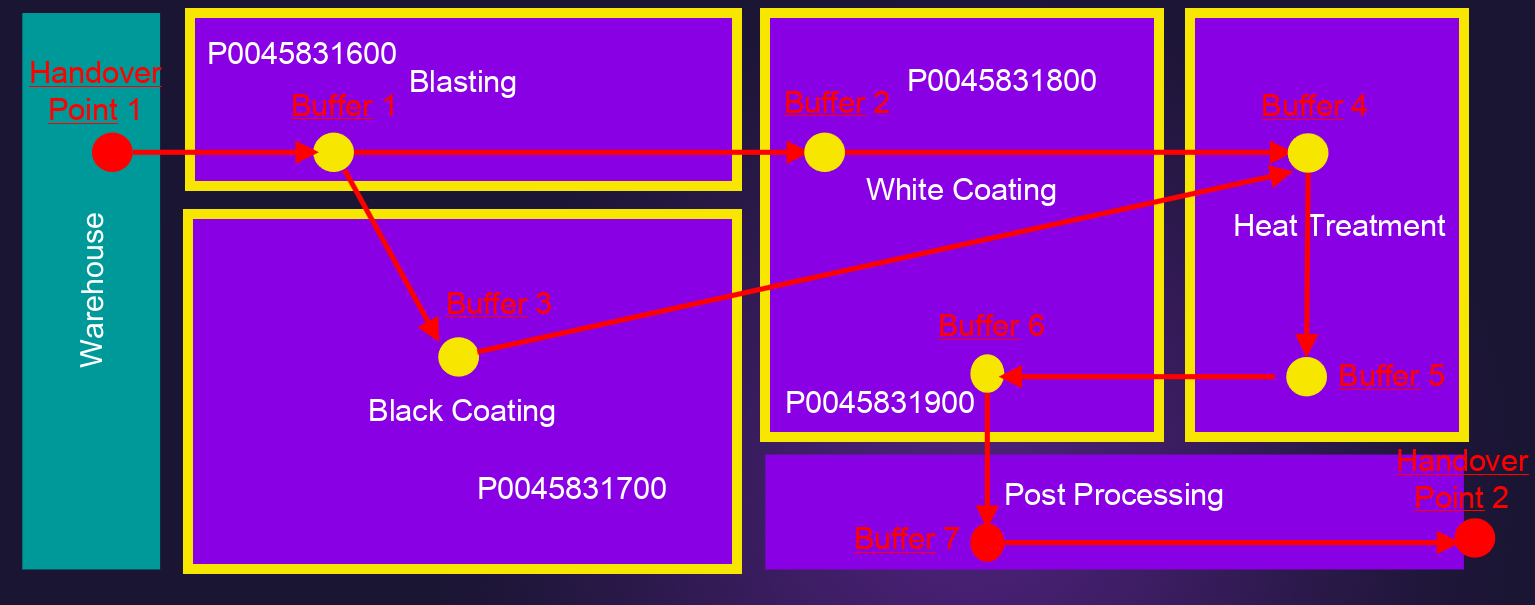
\includegraphics[width=\textwidth]{imagesse/assistantrouting}
\end{frame}

\begin{frame}
\frametitle{Datasets}
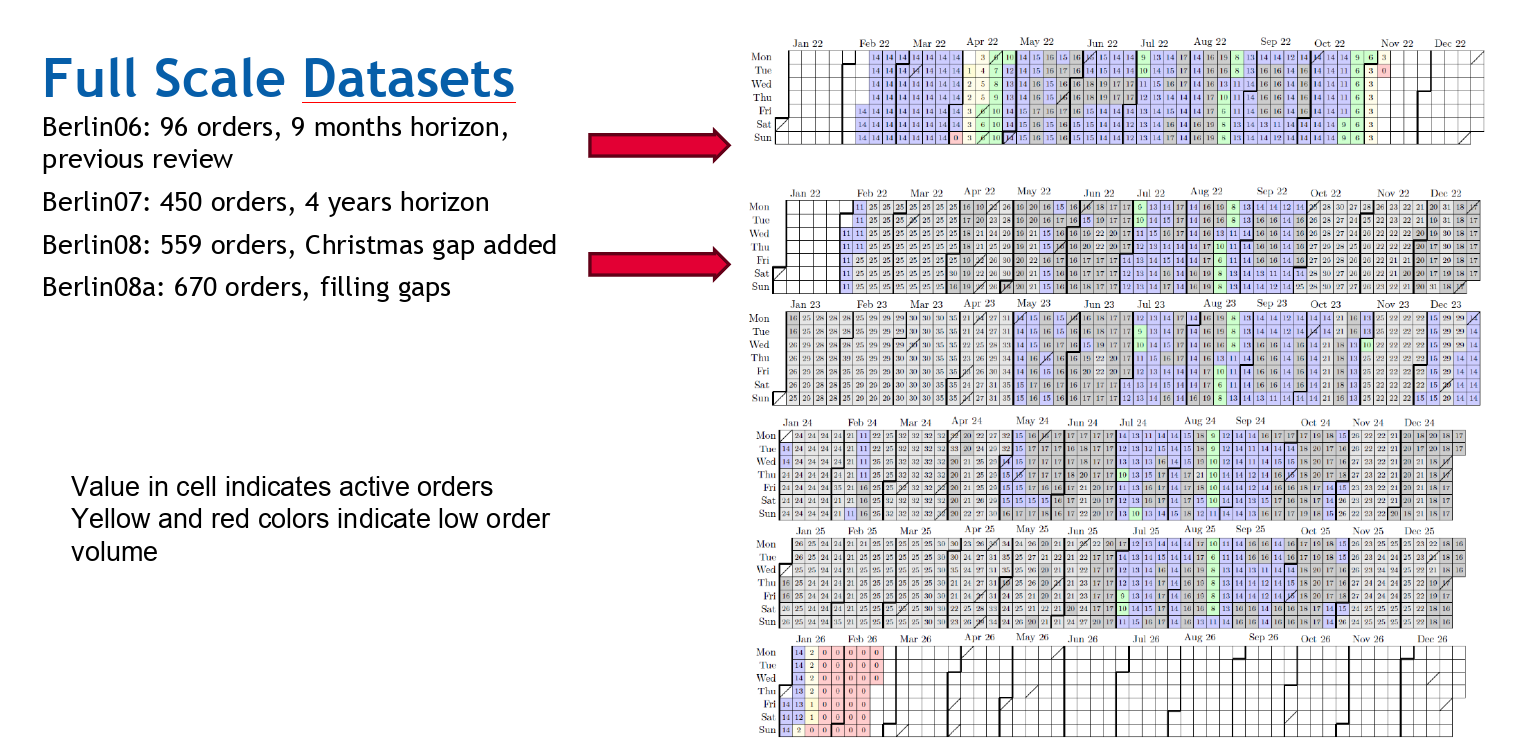
\includegraphics[width=\textwidth]{imagesse/assistantfullscaledatasets}
\end{frame}

\begin{frame}
\frametitle{Optimizer High Level Structure}
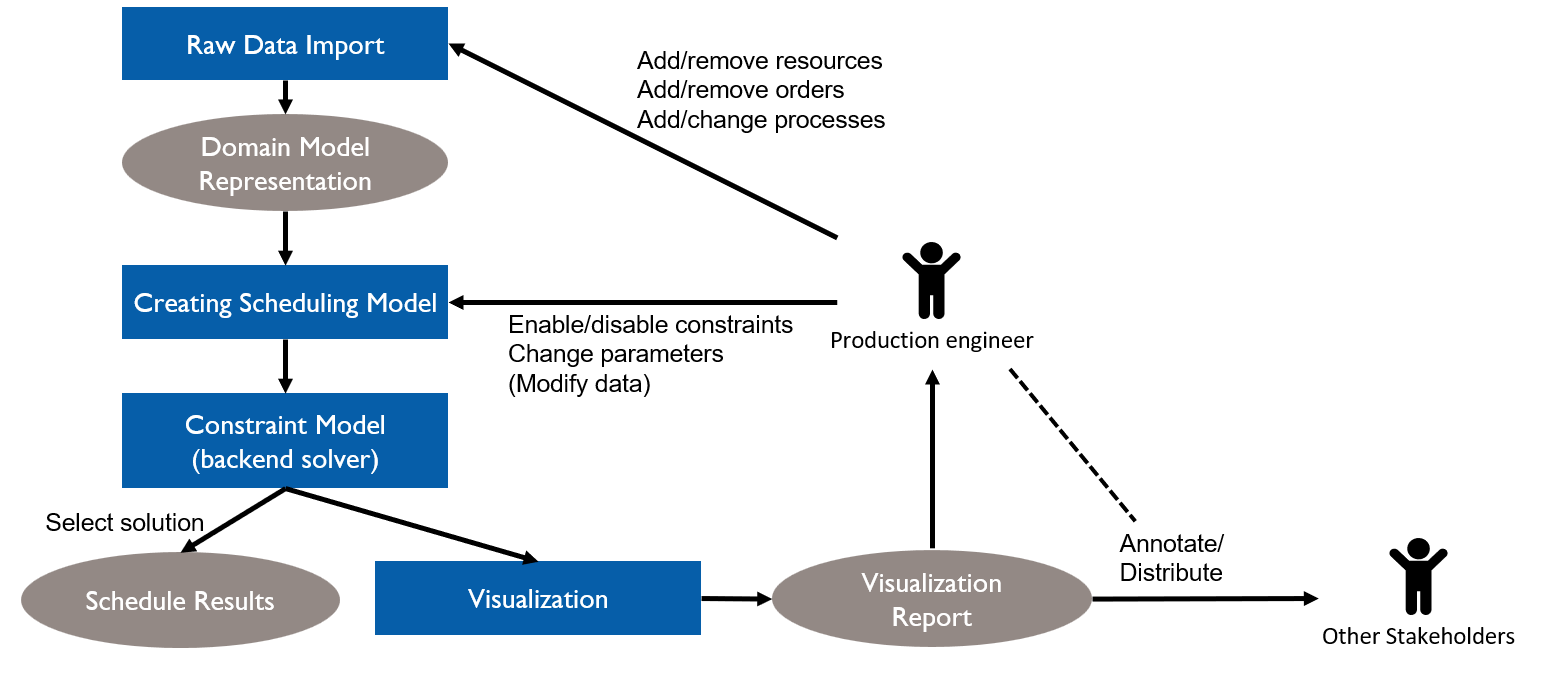
\includegraphics[width=.9\textwidth]{imagesse/overview}
\end{frame}

\begin{frame}
\frametitle{Raw Data - Manual Data Entry Causes Problems}
\begin{columns}
\begin{column}{0.5\textwidth}
\begin{itemize}
\item Raw data come from spreadsheet
\begin{itemize}
\item 20 tabs
\end{itemize}
\item Excel is a particularly bad input data format
\item Realistic, not real data
\item Created by hand/automatically from existing test scenarios
\item Series of files Berlin01 - Berlin05 were too inconsistent to run
\item Berlin06 still contains some errors
\item Optimizer explains all issues that it finds
\end{itemize}
\end{column}
\begin{column}{0.5\textwidth}
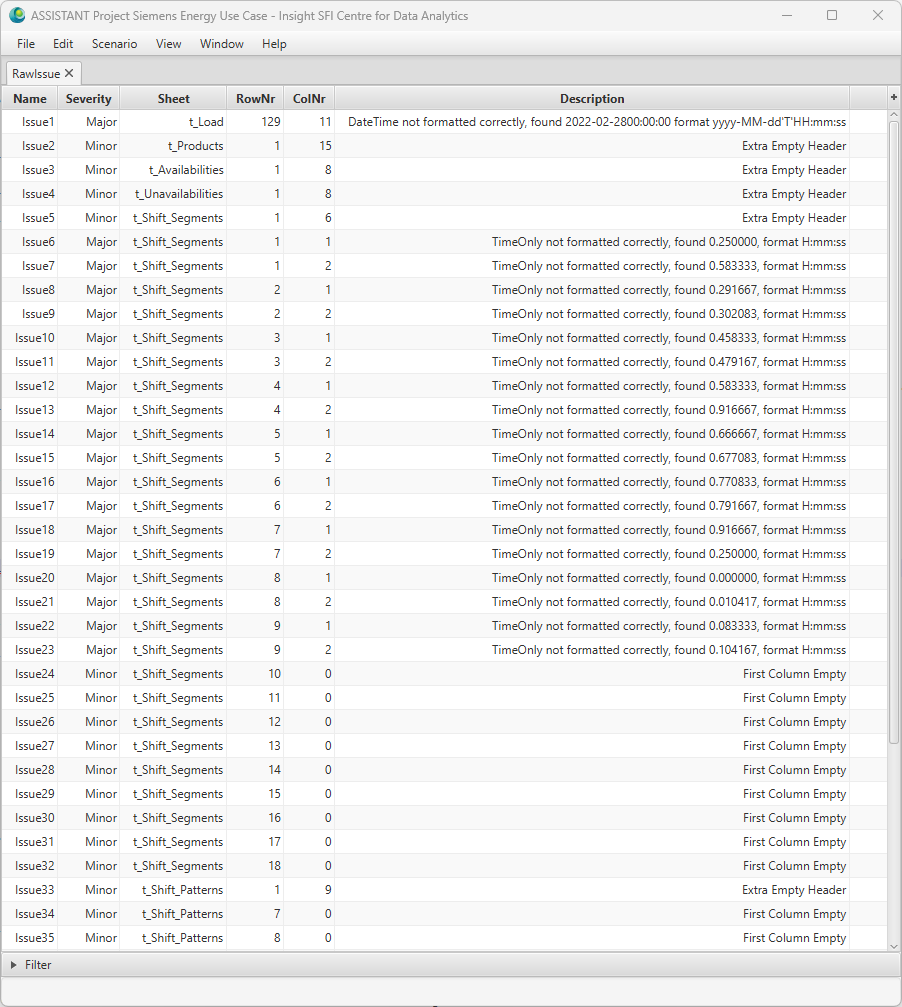
\includegraphics[width=.85\textwidth]{imagesse/rawerror}
\end{column}
\end{columns}
\end{frame}

\begin{frame}
\frametitle{Domain Model - Knowledge Graph}
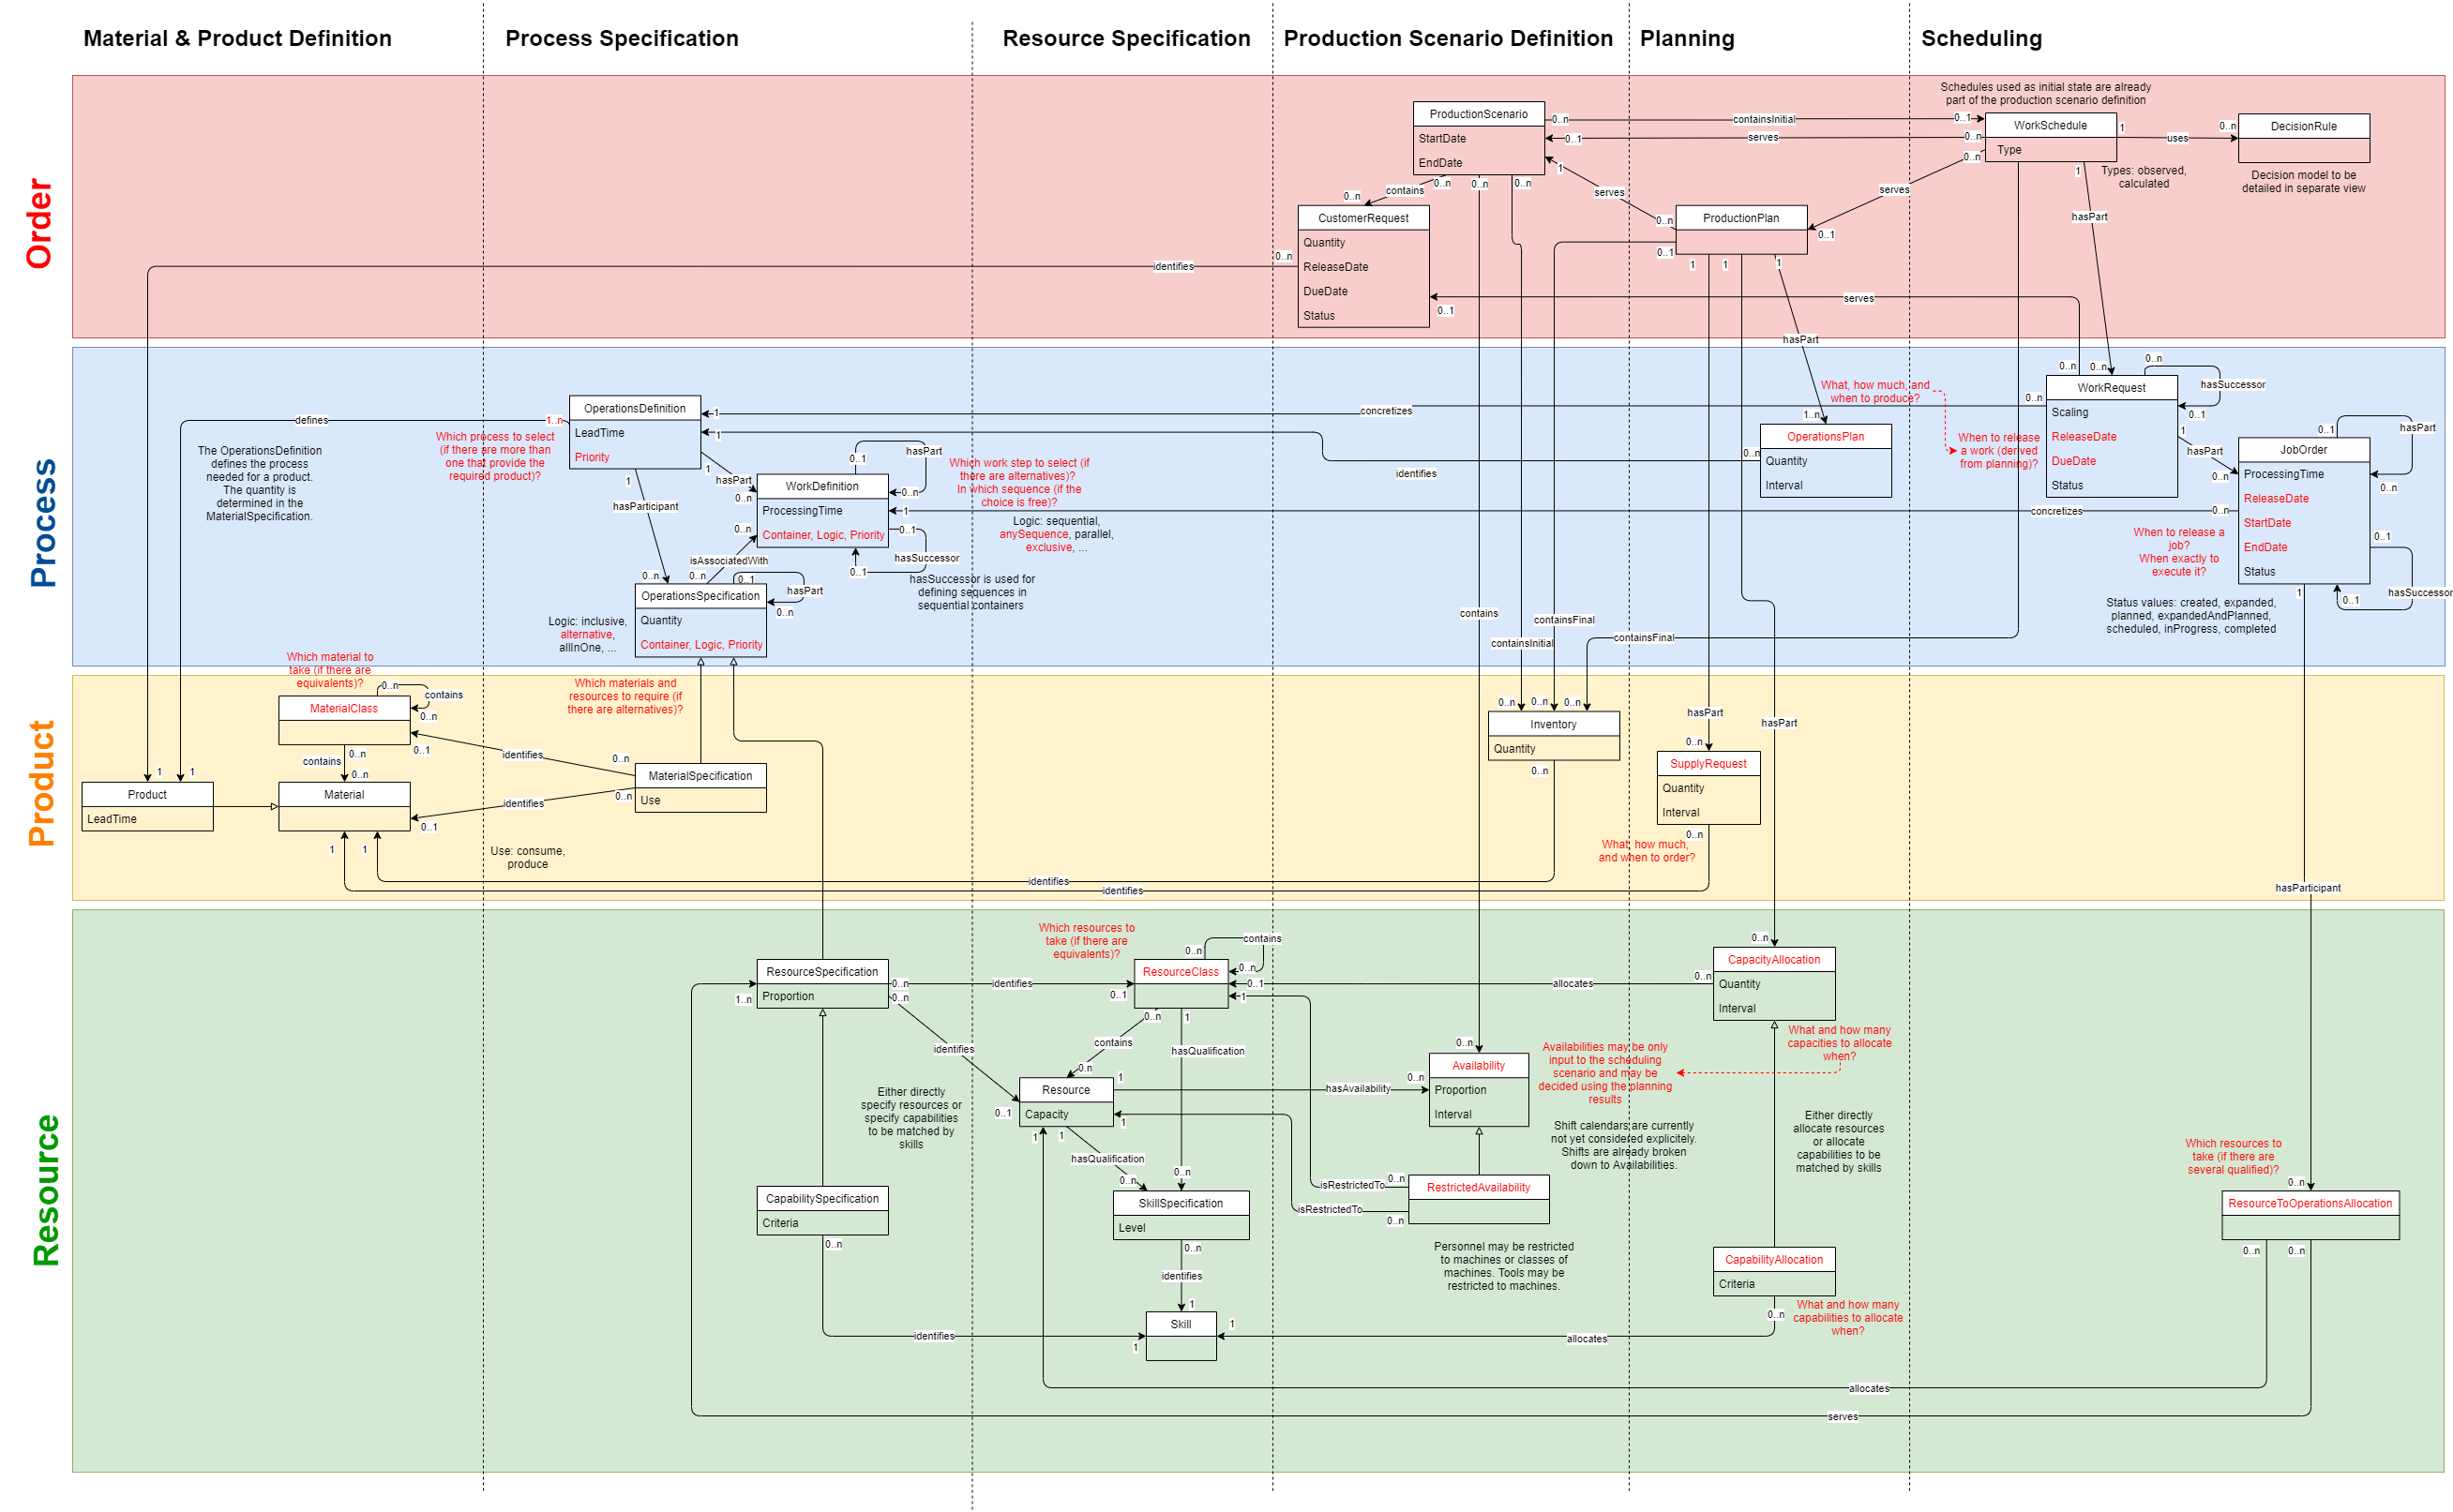
\includegraphics[width=.8\textwidth]{imagesse/DomainModel}
\end{frame}

\begin{frame}
\frametitle{Single Solution for Berlin 08a - Shows Only 20\% of Tasks in Model}
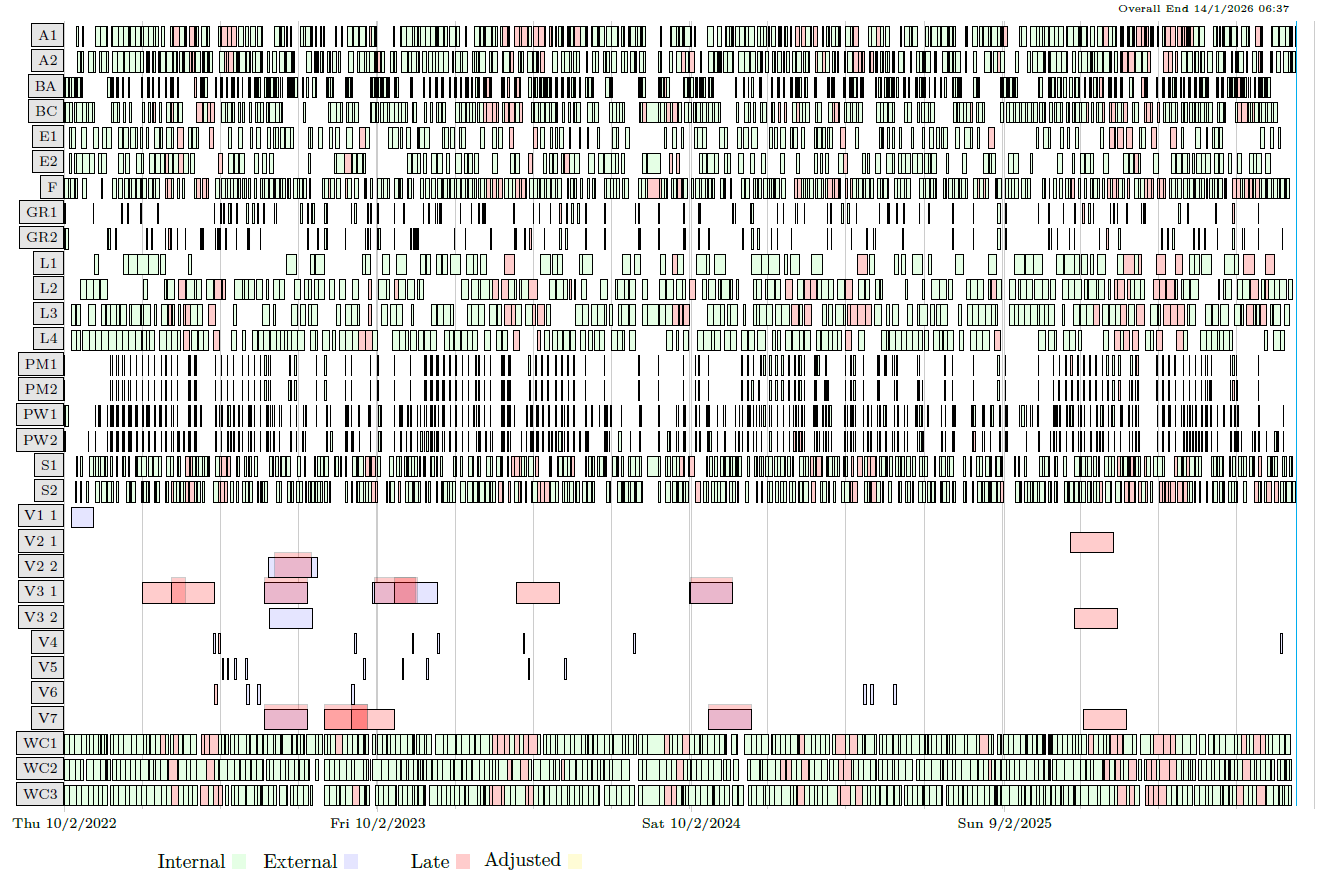
\includegraphics[width=.75\textwidth]{imagesse/solution08apref2}
\end{frame}

\begin{frame}
\frametitle{Implementation}
\begin{itemize}
\item Requirement capture done inside project
\item Data checking/cleaning most time consuming aspect
\item Some specified functionality was rejected by Betriebsrat
\item Built in Java
\item Uses IBM's CPO back-end
\item 120k LoC, 110k generated, 3k solver
\item Outperforms both 
\begin{itemize}
\item Current in-house tool
\item Simulation based tool based on commercial simulator 
\end{itemize}
\item System installed at SE site, but not in daily use
\end{itemize}
\end{frame}


\begin{frame}
\frametitle{CPO Keeps on Trucking}
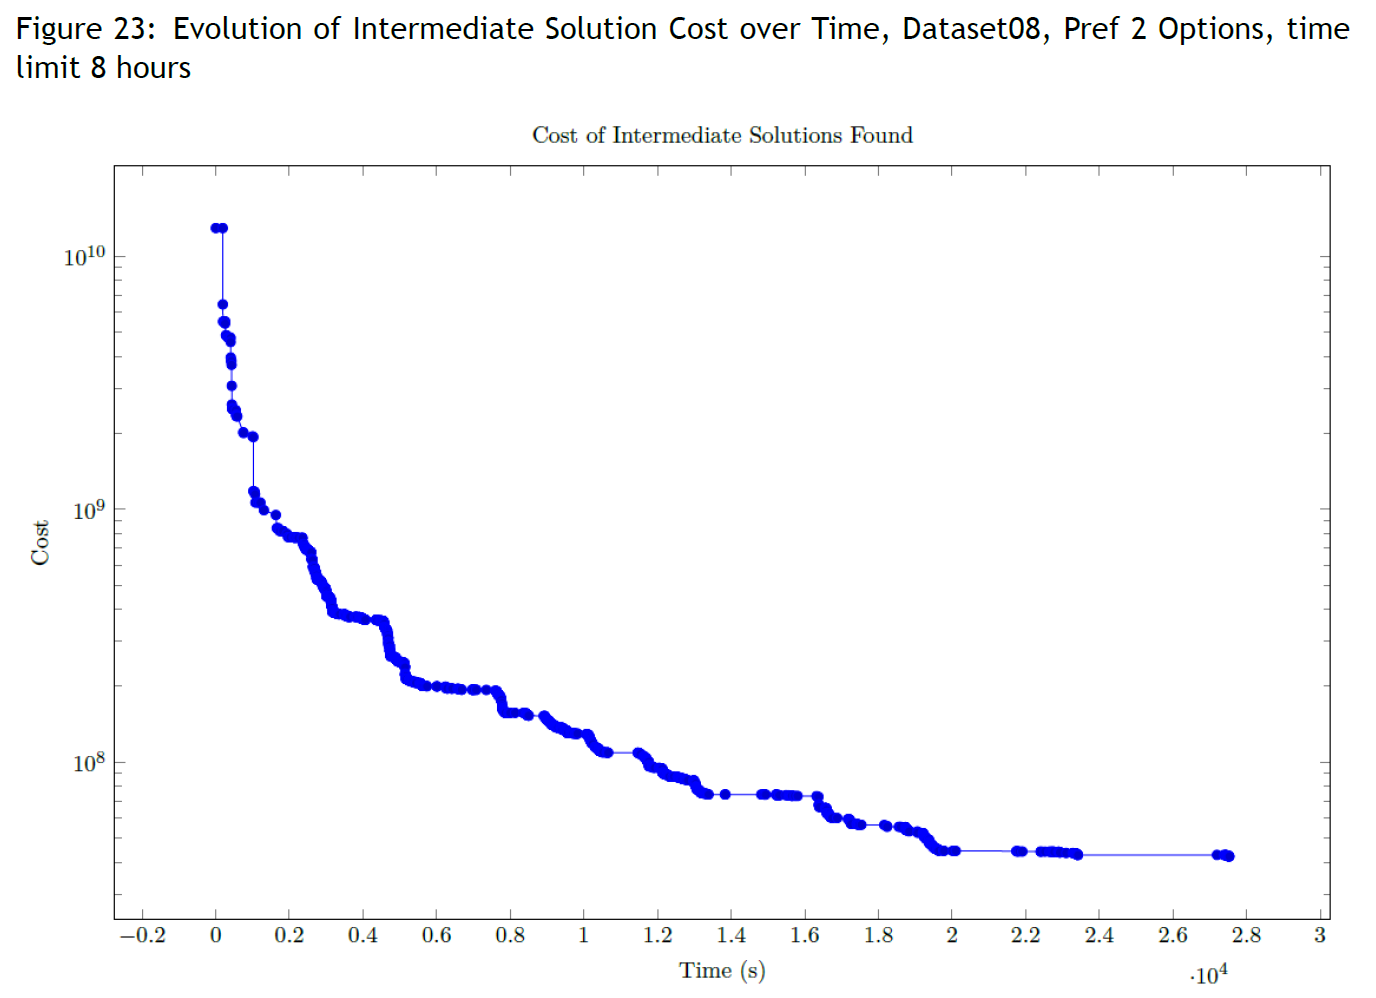
\includegraphics[width=.65\textwidth]{imagesse/improving}
\end{frame}

\begin{frame}
\frametitle{Conclusion}
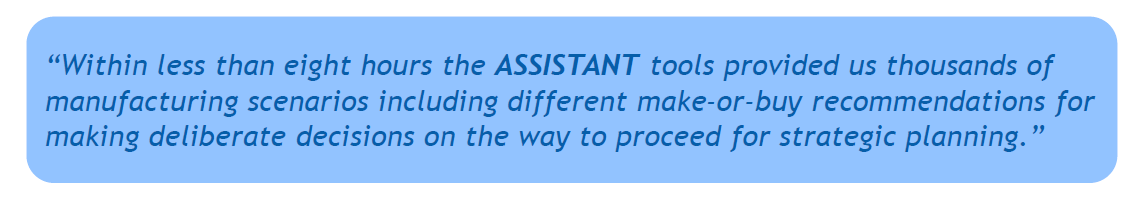
\includegraphics[width=.9\textwidth]{imagesse/quote}

{\tiny Siemens SE final project review assessment}
\end{frame}



